\section[DMAT]{Introduction to pbdDMAT and the DMAT Structure}

\hidenum
\begin{frame}[noframenumbering]
\frametitle{Contents}
 \tableofcontents[currentsection,hideothersubsections,sectionstyle=show/hide]
\end{frame}
\shownum

\subsection{Introduction to Distributed Matrices}

\begin{frame}
  \begin{block}{Distributed Matrices}\pause
  Most problems in data science are matrix algebra problems, so:
  \begin{center}
  $\text{Distributed matrices} \implies \text{Handle Bigger data}$
  \end{center}
  \end{block}
\end{frame}


\begin{frame}[fragile]
  \begin{block}{Distributed Matrices}\pause
  High level OOP allows \emph{native} serial R syntax:
  \begin{lstlisting}
x <- x[-1, 2:5]
x <- log(abs(x) + 1)
xtx <- t(x) %*% x
ans <- svd(solve(xtx))
  \end{lstlisting}
  \vspace{.4cm}
  However\dots
  \end{block}
\end{frame}


\begin{frame}
  \begin{block}{Distributed Matrices}\pause
  DMAT:
    \begin{itemize}
     \item \textbf{D}istributed \textbf{MAT}rix data structure.
     \item No single processor should hold all of the data.
     \item Block-cyclic matrix distributed across a 2-dimensional grid of processors.
     \item Very robust, but confusing data structure.
    \end{itemize}
  \end{block}
\end{frame}



\begin{frame}
\begin{block}{Distributed Matrices}
\begin{figure}[ht]
        \centering
        \begin{subfigure}[b]{0.3\textwidth}
                \centering
                
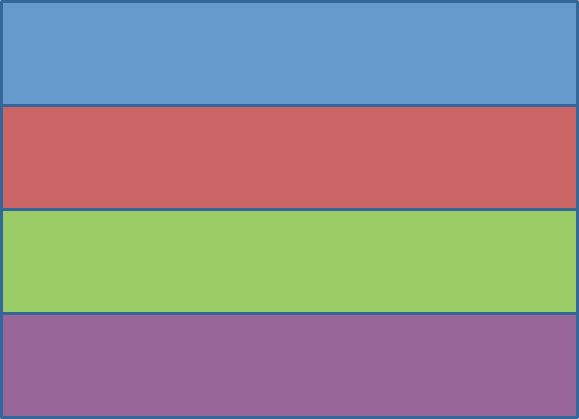
\includegraphics[height=5cm,width=\textwidth]{../common/pics/dmat_block}
                \caption{Block}
        \end{subfigure}
        \hspace{.1cm}
        \begin{subfigure}[b]{0.3\textwidth}
                \centering
                
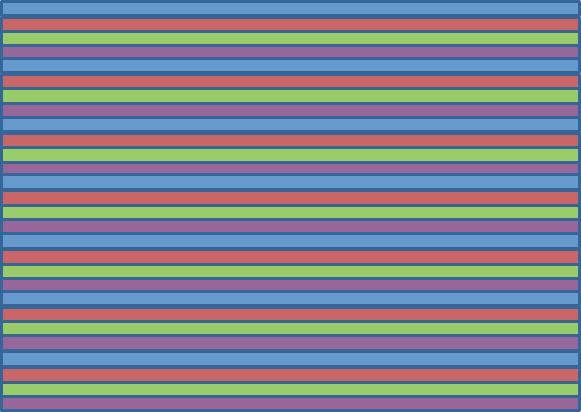
\includegraphics[height=5cm,width=\textwidth]{../common/pics/dmat_cyclic}
                \caption{Cyclic}
        \end{subfigure}
        \hspace{.01cm}
        \begin{subfigure}[b]{0.3\textwidth}
                \centering
                
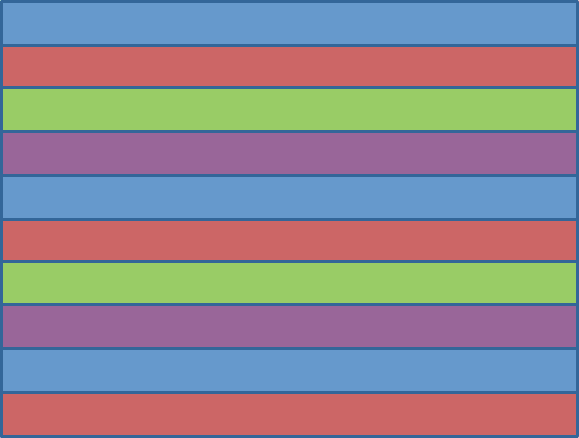
\includegraphics[height=5cm,width=\textwidth]{../common/pics/dmat_blockcyclic}
                \caption{Block-Cyclic}
        \end{subfigure}
        \caption{Matrix Distribution Schemes}\label{fig:dmat1d}
\end{figure}
\end{block}
\end{frame}



\begin{frame}
\begin{block}{Distributed Matrices}
\begin{figure}[ht]
        \centering
        \begin{subfigure}[b]{0.3\textwidth}
                \centering
                
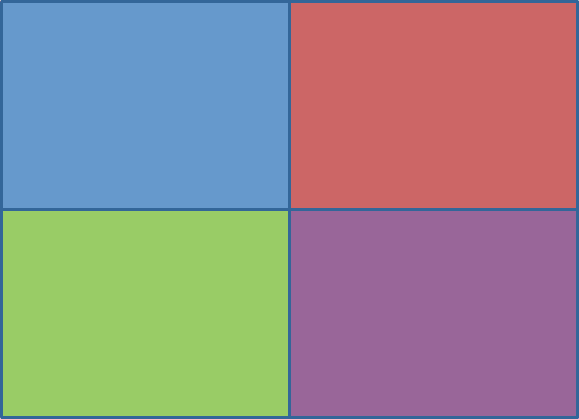
\includegraphics[height=5cm,width=\textwidth]{../common/pics/dmat_block2d}
                \caption{2d Block}
        \end{subfigure}%
        \hspace{.1cm}
        \begin{subfigure}[b]{0.3\textwidth}
                \centering
                
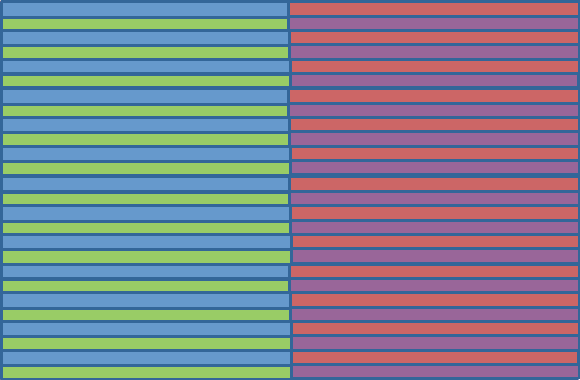
\includegraphics[height=5cm,width=\textwidth]{../common/pics/dmat_cyclic2d}
                \caption{2d Cyclic}
        \end{subfigure}
        \hspace{.01cm}
        \begin{subfigure}[b]{0.3\textwidth}
                \centering
                
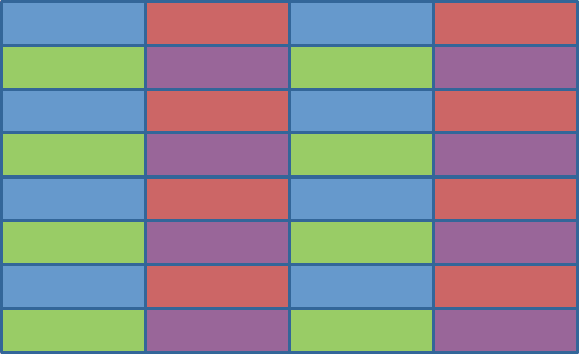
\includegraphics[height=5cm,width=\textwidth]{../common/pics/dmat_blockcyclic2d}
                \caption{2d Block-Cyclic}
        \end{subfigure}
        \caption{Matrix Distribution Schemes Onto a 2-Dimensional 
Grid}\label{fig:dmat2d}
\end{figure}
\end{block}
\end{frame}



\begin{frame}
\begin{block}{Processor Grid Shapes}
\begin{table}[ht]
        \centering
        \begin{subfigure}[b]{0.23\textwidth}
                \centering
              $\left[\begin{tabular}{l}
                  0 \\ 1 \\ 2 \\ 3 \\ 4 \\ 5
                \end{tabular}\right]^T$
                \caption{$1\times 6$}
        \end{subfigure}
        \begin{subfigure}[b]{0.23\textwidth}
                \centering
                $\left[\begin{tabular}{lll}
                  0 & 1 & 2\\
                  3 & 4 & 5
                \end{tabular}\right]$
                \caption{$2\times 3$}
        \end{subfigure}%
        \begin{subfigure}[b]{0.23\textwidth}
                \centering
              $\left[\begin{tabular}{ll}
                  0 & 1 \\
                  2 & 3\\
                  4 & 5
                \end{tabular}\right]$
                \caption{$3\times 2$}
        \end{subfigure}
        \begin{subfigure}[b]{0.23\textwidth}
                \centering
              $\left[\begin{tabular}{l}
                  0 \\ 1 \\ 2 \\ 3 \\ 4 \\ 5
                \end{tabular}\right]$
                \caption{$6\times 1$}
        \end{subfigure}
        \caption{Processor Grid Shapes with 6 Processors}\label{fig:gridshapes}
\end{table}
\end{block}
\end{frame}





\begin{frame}
  \begin{block}{Distributed Matrices}\pause
  The data structure is a special R class (in the OOP sense) called 
\code{ddmatrix}.  It is the ``under the rug'' storage for a block-cyclic matrix 
distributed onto a 2-dimensional processor grid.\\[.4cm]
{\tiny
\begin{align*}
\hspace{.1cm}\text{\code{ddmatrix}}&=\begin{cases}
 $\textbf{Data}$ & $S4 local submatrix, an R matrix$\\
 $\textbf{dim}$ & $S4 dimension of the global matrix, a numeric pair$\\
 $\textbf{ldim}$ & $S4 dimension of the local submatrix, a numeric pair$\\
 $\textbf{bldim}$ & $S4 ScaLAPACK blocking factor, a numeric pair$\\
 $\textbf{CTXT}$ & $S4 BLACS context, an numeric singleton$
 \end{cases}
\end{align*}
}with prototype{\tiny
\begin{align*}
\hspace{-2.9cm}\text{\code{new("ddmatrix")}}&=\begin{cases}
 $\textbf{Data}$ & =\text{\code{matrix(0.0)}}\\
 $\textbf{dim}$ & =\text{\code{c(1,1)}}\\
 $\textbf{ldim}$ & =\text{\code{c(1,1)}}\\
 $\textbf{bldim}$ & =\text{\code{c(1,1)}}\\
 $\textbf{CTXT}$ & =\text{\code{0.0}}
 \end{cases}
\end{align*}
}
  \end{block}
\end{frame}


\begin{frame}
  \begin{block}{Distributed Matrices:  The Data Structure}\pause
      Example:  an $9\times 9$ matrix is distributed with a ``block-cycling'' 
factor of $2\times 2$ on a $2\times 2$ processor grid:
      \begin{center}
      \begin{minipage}{.45\textwidth}
      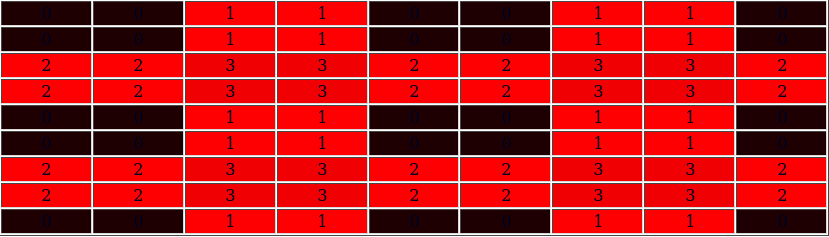
\includegraphics[width=5cm, height=4cm]{../common/pics/dmat_dist}  
      \end{minipage}\hspace{.1cm}
      \begin{minipage}{.45\textwidth}
      \begin{center}
      \begin{align*}
        &=\begin{cases}
        $\textbf{Data}$ & =\text{\code{matrix(\dots)}}\\
        $\textbf{dim}$ & =\text{\code{c(9, 9)}}\\
        $\textbf{ldim}$ & =\text{\code{c(\dots)}}\\
        $\textbf{bldim}$ & =\text{\code{c(2, 2)}}\\
        $\textbf{CTXT}$ & =0
        \end{cases}
        \end{align*}
      \end{center}
      \end{minipage}
      \end{center}
    {\small See \url{http://acts.nersc.gov/scalapack/hands-on/datadist.html}}
  \end{block}
\end{frame}

  
  
  

\subsection{DMAT Distributions}




\begin{frame}
\begin{exampleblock}{Understanding Dmat: Global Matrix}
\begin{align*}
x &= \left[
      \begin{array}{lllllllll}
      x_{11} & x_{12} & x_{13} & x_{14} & x_{15} & x_{16} & x_{17} & x	_{18} & x_{19}\\
      x_{21} & x_{22} & x_{23} & x_{24} & x_{25} & x_{26} & x_{27} & x	_{28} & x_{29}\\
      x_{31} & x_{32} & x_{33} & x_{34} & x_{35} & x_{36} & x_{37} & x	_{38} & x_{39}\\
      x_{41} & x_{42} & x_{43} & x_{44} & x_{45} & x_{46} & x_{47} & x	_{48} & x_{49}\\
      x_{51} & x_{52} & x_{53} & x_{54} & x_{55} & x_{56} & x_{57} & x	_{58} & x_{59}\\
      x_{61} & x_{62} & x_{63} & x_{64} & x_{65} & x_{66} & x_{67} & x	_{68} & x_{69}\\
      x_{71} & x_{72} & x_{73} & x_{74} & x_{75} & x_{76} & x_{77} & x	_{78} & x_{79}\\
      x_{81} & x_{82} & x_{83} & x_{84} & x_{85} & x_{86} & x_{87} & x	_{88} & x_{89}\\
      x_{91} & x_{92} & x_{93} & x_{94} & x_{95} & x_{96} & x_{97} & x	_{98} & x_{99}
      \end{array}
\right]_{9\times 9}
\end{align*}
\end{exampleblock}
\end{frame}



\begin{frame}
\begin{exampleblock}{DMAT:  1-dimensional Row Block}
\begin{align*}
x &= \left[
      \begin{array}{lllllllll}
      \color{g11}x_{11} & \color{g11}x_{12} & \color{g11}x_{13} & 
\color{g11}x_{14} & \color{g11}x_{15} & \color{g11}x_{16} & \color{g11}x_{17} & 
\color{g11}x_{18} & \color{g11}x_{19}\\
      \color{g11}x_{21} & \color{g11}x_{22} & \color{g11}x_{23} & 
\color{g11}x_{24} & \color{g11}x_{25} & \color{g11}x_{26} & \color{g11}x_{27} & 
\color{g11}x_{28} & \color{g11}x_{29}\\
      \color{g11}x_{31} & \color{g11}x_{32} & \color{g11}x_{33} & 
\color{g11}x_{34} & \color{g11}x_{35} & \color{g11}x_{36} & \color{g11}x_{37} & 
\color{g11}x_{38} & \color{g11}x_{39}\\\hline
      \color{g12}x_{41} & \color{g12}x_{42} & \color{g12}x_{43} & 
\color{g12}x_{44} & \color{g12}x_{45} & \color{g12}x_{46} & \color{g12}x_{47} & 
\color{g12}x_{48} & \color{g12}x_{49}\\
      \color{g12}x_{51} & \color{g12}x_{52} & \color{g12}x_{53} & 
\color{g12}x_{54} & \color{g12}x_{55} & \color{g12}x_{56} & \color{g12}x_{57} & 
\color{g12}x_{58} & \color{g12}x_{59}\\
      \color{g12}x_{61} & \color{g12}x_{62} & \color{g12}x_{63} & 
\color{g12}x_{64} & \color{g12}x_{65} & \color{g12}x_{66} & \color{g12}x_{67} & 
\color{g12}x_{68} & \color{g12}x_{69}\\\hline
      \color{g13}x_{71} & \color{g13}x_{72} & \color{g13}x_{73} & 
\color{g13}x_{74} & \color{g13}x_{75} & \color{g13}x_{76} & \color{g13}x_{77} & 
\color{g13}x_{78} & \color{g13}x_{79}\\
      \color{g13}x_{81} & \color{g13}x_{82} & \color{g13}x_{83} & 
\color{g13}x_{84} & \color{g13}x_{85} & \color{g13}x_{86} & \color{g13}x_{87} & 
\color{g13}x_{88} & \color{g13}x_{89}\\
      \color{g13}x_{91} & \color{g13}x_{92} & \color{g13}x_{93} & 
\color{g13}x_{94} & \color{g13}x_{95} & \color{g13}x_{96} & \color{g13}x_{97} & 
\color{g13}x_{98} & \color{g13}x_{99}\\
      \end{array}
\right]_{9\times 9}
\end{align*}
\vspace{-.6cm}
\begin{align*}
\text{Processor grid = }\left|
      \begin{array}{l}
      \color{g11}0 \\
      \color{g12}1 \\
      \color{g13}2 \\
      \color{g21}3
      \end{array}
\right| &= 
\left|
      \begin{tabular}{l}
      \color{g11}(0,0) \\
      \color{g12}(1,0) \\
      \color{g13}(2,0) \\
      \color{g21}(3,0) 
      \end{tabular}
\right|
\end{align*}
\end{exampleblock}
\end{frame}





\begin{frame}
\begin{exampleblock}{DMAT: 2-dimensional Row Block}
\begin{align*}
x &= \left[
      \begin{array}{lllll|llll}
      \color{g11}x_{11} & \color{g11}x_{12} & \color{g11}x_{13} & 
\color{g11}x_{14} & \color{g11}x_{15} & \color{g12}x_{16} & \color{g12}x_{17} & 
\color{g12}x_{18} & \color{g12}x_{19}\\
      \color{g11}x_{21} & \color{g11}x_{22} & \color{g11}x_{23} & 
\color{g11}x_{24} & \color{g11}x_{25} & \color{g12}x_{26} & \color{g12}x_{27} & 
\color{g12}x_{28} & \color{g12}x_{29}\\
      \color{g11}x_{31} & \color{g11}x_{32} & \color{g11}x_{33} & 
\color{g11}x_{34} & \color{g11}x_{35} & \color{g12}x_{36} & \color{g12}x_{37} & 
\color{g12}x_{38} & \color{g12}x_{39}\\
      \color{g11}x_{41} & \color{g11}x_{42} & \color{g11}x_{43} & 
\color{g11}x_{44} & \color{g11}x_{45} & \color{g12}x_{46} & \color{g12}x_{47} & 
\color{g12}x_{48} & \color{g12}x_{49}\\
      \color{g11}x_{51} & \color{g11}x_{52} & \color{g11}x_{53} & 
\color{g11}x_{54} & \color{g11}x_{55} & \color{g12}x_{56} & \color{g12}x_{57} & 
\color{g12}x_{58} & \color{g12}x_{59}\\\hline
      \color{g13}x_{61} & \color{g13}x_{62} & \color{g13}x_{63} & 
\color{g13}x_{64} & \color{g13}x_{65} & \color{g21}x_{66} & \color{g21}x_{67} & 
\color{g21}x_{68} & \color{g21}x_{69}\\
      \color{g13}x_{71} & \color{g13}x_{72} & \color{g13}x_{73} & 
\color{g13}x_{74} & \color{g13}x_{75} & \color{g21}x_{76} & \color{g21}x_{77} & 
\color{g21}x_{78} & \color{g21}x_{79}\\
      \color{g13}x_{81} & \color{g13}x_{82} & \color{g13}x_{83} & 
\color{g13}x_{84} & \color{g13}x_{85} & \color{g21}x_{86} & \color{g21}x_{87} & 
\color{g21}x_{88} & \color{g21}x_{89}\\
      \color{g13}x_{91} & \color{g13}x_{92} & \color{g13}x_{93} & 
\color{g13}x_{94} & \color{g13}x_{95} & \color{g21}x_{96} & \color{g21}x_{97} & 
\color{g21}x_{98} & \color{g21}x_{99}\\
      \end{array}
\right]_{9\times 9}
\end{align*}
\begin{align*}
\text{Processor grid = }\left|
      \begin{array}{ll}
      \color{g11}0 & \color{g12}1 \\
      \color{g13}2 & \color{g21}3
      \end{array}
\right| &= 
\left|
      \begin{tabular}{lll}
      \color{g11}(0,0) & \color{g12}(0,1) \\
      \color{g13}(1,0) & \color{g21}(1,1) 
      \end{tabular}
\right|
\end{align*}
\end{exampleblock}
\end{frame}



\begin{frame}
\begin{exampleblock}{DMAT: 1-dimensional Row Cyclic}
\begin{align*}
x &= \left[
      \begin{array}{lllllllll}
      \color{g11}x_{11} & \color{g11}x_{12} & \color{g11}x_{13} & 
\color{g11}x_{14} & \color{g11}x_{15} & \color{g11}x_{16} & \color{g11}x_{17} & 
\color{g11}x_{18} & \color{g11}x_{19}\\\hline
      \color{g12}x_{21} & \color{g12}x_{22} & \color{g12}x_{23} & 
\color{g12}x_{24} & \color{g12}x_{25} & \color{g12}x_{26} & \color{g12}x_{27} & 
\color{g12}x_{28} & \color{g12}x_{29}\\\hline
      \color{g13}x_{31} & \color{g13}x_{32} & \color{g13}x_{33} & 
\color{g13}x_{34} & \color{g13}x_{35} & \color{g13}x_{36} & \color{g13}x_{37} & 
\color{g13}x_{38} & \color{g13}x_{39}\\\hline
      \color{g21}x_{41} & \color{g21}x_{42} & \color{g21}x_{43} & 
\color{g21}x_{44} & \color{g21}x_{45} & \color{g21}x_{46} & \color{g21}x_{47} & 
\color{g21}x_{48} & \color{g21}x_{49}\\\hline
      \color{g11}x_{51} & \color{g11}x_{52} & \color{g11}x_{53} & 
\color{g11}x_{54} & \color{g11}x_{55} & \color{g11}x_{56} & \color{g11}x_{57} & 
\color{g11}x_{58} & \color{g11}x_{59}\\\hline
      \color{g12}x_{61} & \color{g12}x_{62} & \color{g12}x_{63} & 
\color{g12}x_{64} & \color{g12}x_{65} & \color{g12}x_{66} & \color{g12}x_{67} & 
\color{g12}x_{68} & \color{g12}x_{69}\\\hline
      \color{g13}x_{71} & \color{g13}x_{72} & \color{g13}x_{73} & 
\color{g13}x_{74} & \color{g13}x_{75} & \color{g13}x_{76} & \color{g13}x_{77} & 
\color{g13}x_{78} & \color{g13}x_{79}\\\hline
      \color{g21}x_{81} & \color{g21}x_{82} & \color{g21}x_{83} & 
\color{g21}x_{84} & \color{g21}x_{85} & \color{g21}x_{86} & \color{g21}x_{87} & 
\color{g21}x_{88} & \color{g21}x_{89}\\\hline
      \color{g11}x_{91} & \color{g11}x_{92} & \color{g11}x_{93} & 
\color{g11}x_{94} & \color{g11}x_{95} & \color{g11}x_{96} & \color{g11}x_{97} & 
\color{g11}x_{98} & \color{g11}x_{99}\\
      \end{array}
\right]_{9\times 9}
\end{align*}
\vspace{-.6cm}
\begin{align*}
\text{Processor grid = }\left|
      \begin{array}{l}
      \color{g11}0 \\
      \color{g12}1 \\
      \color{g13}2 \\
      \color{g21}3
      \end{array}
\right| &= 
\left|
      \begin{tabular}{lll}
      \color{g11}(0,0) \\
      \color{g12}(1,0) \\
      \color{g13}(2,0) \\
      \color{g21}(3,0) 
      \end{tabular}
\right|
\end{align*}
\end{exampleblock}
\end{frame}



\begin{frame}
\begin{exampleblock}{DMAT: 2-dimensional Row Cyclic}
\begin{align*}
x &= \left[
      \begin{array}{lllll|llll}
      \color{g11}x_{11} & \color{g11}x_{12} & \color{g11}x_{13} & 
\color{g11}x_{14} & \color{g11}x_{15} & \color{g12}x_{16} & \color{g12}x_{17} & 
\color{g12}x_{18} & \color{g12}x_{19}\\\hline
      \color{g13}x_{21} & \color{g13}x_{22} & \color{g13}x_{23} & 
\color{g13}x_{24} & \color{g13}x_{25} & \color{g21}x_{26} & \color{g21}x_{27} & 
\color{g21}x_{28} & \color{g21}x_{29}\\\hline
      \color{g11}x_{31} & \color{g11}x_{32} & \color{g11}x_{33} & 
\color{g11}x_{34} & \color{g11}x_{35} & \color{g12}x_{36} & \color{g12}x_{37} & 
\color{g12}x_{38} & \color{g12}x_{39}\\\hline
      \color{g13}x_{41} & \color{g13}x_{42} & \color{g13}x_{43} & 
\color{g13}x_{44} & \color{g13}x_{45} & \color{g21}x_{46} & \color{g21}x_{47} & 
\color{g21}x_{48} & \color{g21}x_{49}\\\hline
      \color{g11}x_{51} & \color{g11}x_{52} & \color{g11}x_{53} & 
\color{g11}x_{54} & \color{g11}x_{55} & \color{g12}x_{56} & \color{g12}x_{57} & 
\color{g12}x_{58} & \color{g12}x_{59}\\\hline
      \color{g13}x_{61} & \color{g13}x_{62} & \color{g13}x_{63} & 
\color{g13}x_{64} & \color{g13}x_{65} & \color{g21}x_{66} & \color{g21}x_{67} & 
\color{g21}x_{68} & \color{g21}x_{69}\\\hline
      \color{g11}x_{71} & \color{g11}x_{72} & \color{g11}x_{73} & 
\color{g11}x_{74} & \color{g11}x_{75} & \color{g12}x_{76} & \color{g12}x_{77} & 
\color{g12}x_{78} & \color{g12}x_{79}\\\hline
      \color{g13}x_{81} & \color{g13}x_{82} & \color{g13}x_{83} & 
\color{g13}x_{84} & \color{g13}x_{85} & \color{g21}x_{86} & \color{g21}x_{87} & 
\color{g21}x_{88} & \color{g21}x_{89}\\\hline
      \color{g11}x_{91} & \color{g11}x_{92} & \color{g11}x_{93} & 
\color{g11}x_{94} & \color{g11}x_{95} & \color{g12}x_{96} & \color{g12}x_{97} & 
\color{g12}x_{98} & \color{g12}x_{99}\\
      \end{array}
\right]_{9\times 9}
\end{align*}
\begin{align*}
\text{Processor grid = }\left|
      \begin{array}{ll}
      \color{g11}0 & \color{g12}1 \\
      \color{g13}2 & \color{g21}3
      \end{array}
\right| &= 
\left|
      \begin{tabular}{lll}
      \color{g11}(0,0) & \color{g12}(0,1) \\
      \color{g13}(1,0) & \color{g21}(1,1) 
      \end{tabular}
\right|
\end{align*}
\end{exampleblock}
\end{frame}




\begin{frame}[shrink]
\begin{exampleblock}{DMAT: 2-dimensional Block-Cyclic}
\begin{align*}
x &= \left[
      \begin{array}{ll|ll|ll|ll|l}
      \color{g11}x_{11} & \color{g11}x_{12} & \color{g12}x_{13} & \color{g12}x_{14} & \color{g11}x_{15} & \color{g11}x_{16} & \color{g12}x_{17} & \color{g12}x_{18} & \color{g11}x_{19}\\
      \color{g11}x_{21} & \color{g11}x_{22} & \color{g12}x_{23} & \color{g12}x_{24} & \color{g11}x_{25} & \color{g11}x_{26} & \color{g12}x_{27} & \color{g12}x_{28} & \color{g11}x_{29}\\\hline
      \color{g13}x_{31} & \color{g13}x_{32} & \color{g21}x_{33} & \color{g21}x_{34} & \color{g13}x_{35} & \color{g13}x_{36} & \color{g21}x_{37} & \color{g21}x_{38} & \color{g13}x_{39}\\
      \color{g13}x_{41} & \color{g13}x_{42} & \color{g21}x_{43} & \color{g21}x_{44} & \color{g13}x_{45} & \color{g13}x_{46} & \color{g21}x_{47} & \color{g21}x_{48} & \color{g13}x_{49}\\\hline
      \color{g11}x_{51} & \color{g11}x_{52} & \color{g12}x_{53} & \color{g12}x_{54} & \color{g11}x_{55} & \color{g11}x_{56} & \color{g12}x_{57} & \color{g12}x_{58} & \color{g11}x_{59}\\
      \color{g11}x_{61} & \color{g11}x_{62} & \color{g12}x_{63} & \color{g12}x_{64} & \color{g11}x_{65} & \color{g11}x_{66} & \color{g12}x_{67} & \color{g12}x_{68} & \color{g11}x_{69}\\\hline
      \color{g13}x_{71} & \color{g13}x_{72} & \color{g21}x_{73} & \color{g21}x_{74} & \color{g13}x_{75} & \color{g13}x_{76} & \color{g21}x_{77} & \color{g21}x_{78} & \color{g13}x_{79}\\
      \color{g13}x_{81} & \color{g13}x_{82} & \color{g21}x_{83} & \color{g21}x_{84} & \color{g13}x_{85} & \color{g13}x_{86} & \color{g21}x_{87} & \color{g21}x_{88} & \color{g13}x_{89}\\\hline
      \color{g11}x_{91} & \color{g11}x_{92} & \color{g12}x_{93} & \color{g12}x_{94} & \color{g11}x_{95} & \color{g11}x_{96} & \color{g12}x_{97} & \color{g12}x_{98} & \color{g11}x_{99}\\
      \end{array}
\right]_{9\times 9}
\end{align*}
\begin{align*}
\text{Processor grid = }\left|
      \begin{array}{ll}
      \color{g11}0 & \color{g12}1 \\
      \color{g13}2 & \color{g21}3
      \end{array}
\right| &= 
\left|
      \begin{tabular}{lll}
      \color{g11}(0,0) & \color{g12}(0,1) \\
      \color{g13}(1,0) & \color{g21}(1,1) 
      \end{tabular}
\right|
\end{align*}
\end{exampleblock}
\end{frame}








\subsection{pbdDMAT}

\begin{frame}[fragile]
  \begin{block}{The \code{DMAT} Data Structure}\pause
    The more complicated the processor grid, the more complicated the distribution.
  \end{block}
\end{frame}


\begin{frame}[shrink]
\begin{exampleblock}{DMAT: 2-dimensional Block-Cyclic with 6 Processors}
\begin{align*}
x &= \left[
      \begin{array}{ll|ll|ll|ll|l}
      \color{g11}x_{11} & \color{g11}x_{12} & \color{g12}x_{13} & \color{g12}x_{14} & \color{g13}x_{15} & \color{g13}x_{16} & \color{g11}x_{17} & \color{g11}x_{18} & \color{g12}x_{19}\\
      \color{g11}x_{21} & \color{g11}x_{22} & \color{g12}x_{23} & \color{g12}x_{24} & \color{g13}x_{25} & \color{g13}x_{26} & \color{g11}x_{27} & \color{g11}x_{28} & \color{g12}x_{29}\\\hline
      \color{g21}x_{31} & \color{g21}x_{32} & \color{g22}x_{33} & \color{g22}x_{34} & \color{g23}x_{35} & \color{g23}x_{36} & \color{g21}x_{37} & \color{g21}x_{38} & \color{g22}x_{39}\\
      \color{g21}x_{41} & \color{g21}x_{42} & \color{g22}x_{43} & \color{g22}x_{44} & \color{g23}x_{45} & \color{g23}x_{46} & \color{g21}x_{47} & \color{g21}x_{48} & \color{g22}x_{49}\\\hline
      \color{g11}x_{51} & \color{g11}x_{52} & \color{g12}x_{53} & \color{g12}x_{54} & \color{g13}x_{55} & \color{g13}x_{56} & \color{g11}x_{57} & \color{g11}x_{58} & \color{g12}x_{59}\\
      \color{g11}x_{61} & \color{g11}x_{62} & \color{g12}x_{63} & \color{g12}x_{64} & \color{g13}x_{65} & \color{g13}x_{66} & \color{g11}x_{67} & \color{g11}x_{68} & \color{g12}x_{69}\\\hline
      \color{g21}x_{71} & \color{g21}x_{72} & \color{g22}x_{73} & \color{g22}x_{74} & \color{g23}x_{75} & \color{g23}x_{76} & \color{g21}x_{77} & \color{g21}x_{78} & \color{g22}x_{79}\\
      \color{g21}x_{81} & \color{g21}x_{82} & \color{g22}x_{83} & \color{g22}x_{84} & \color{g23}x_{85} & \color{g23}x_{86} & \color{g21}x_{87} & \color{g21}x_{88} & \color{g22}x_{89}\\\hline
      \color{g11}x_{91} & \color{g11}x_{92} & \color{g12}x_{93} & \color{g12}x_{94} & \color{g13}x_{95} & \color{g13}x_{96} & \color{g11}x_{97} & \color{g11}x_{98} & \color{g12}x_{99}\\
      \end{array}
\right]_{9\times 9}
\end{align*}
\begin{align*}
\text{Processor grid = }\left|
      \begin{array}{lll}
      \color{g11}0 & \color{g12}1 & \color{g13}2\\
      \color{g21}3 & \color{g22}4 & \color{g23}5
      \end{array}
\right| &= 
\left|
      \begin{tabular}{lll}
      \color{g11}(0,0) & \color{g12}(0,1) & \color{g13}(0,2)\\
      \color{g21}(1,0) & \color{g22}(1,1) & \color{g23}(1,2)
      \end{tabular}
\right|
\end{align*}
\end{exampleblock}
\end{frame}


\begin{frame}[shrink]
\begin{exampleblock}{Understanding DMAT: Local View}
\begin{align*}
\left[
      \begin{array}{ll|ll}
      \color{g11}x_{11} & \color{g11}x_{12} & \color{g11}x_{17} & \color{g11}x_{18}\\
      \color{g11}x_{21} & \color{g11}x_{22} & \color{g11}x_{27} & \color{g11}x_{28}\\\hline
      \color{g11}x_{51} & \color{g11}x_{52} & \color{g11}x_{57} & \color{g11}x_{58}\\
      \color{g11}x_{61} & \color{g11}x_{62} & \color{g11}x_{67} & \color{g11}x_{68}\\\hline
      \color{g11}x_{91} & \color{g11}x_{92} & \color{g11}x_{97} & \color{g11}x_{98}\\
      \end{array}
\right]_{5\times 4}
\left[
      \begin{array}{ll|l}
      \color{g12}x_{13} & \color{g12}x_{14} & \color{g12}x_{19}\\
      \color{g12}x_{23} & \color{g12}x_{24} & \color{g12}x_{29}\\\hline
      \color{g12}x_{53} & \color{g12}x_{54} & \color{g12}x_{59}\\
      \color{g12}x_{63} & \color{g12}x_{64} & \color{g12}x_{69}\\\hline
      \color{g12}x_{93} & \color{g12}x_{94} & \color{g12}x_{99}\\
      \end{array}
\right]_{5\times 3}
\left[
      \begin{array}{ll}
      \color{g13}x_{15} & \color{g13}x_{16}\\
      \color{g13}x_{25} & \color{g13}x_{26}\\\hline
      \color{g13}x_{55} & \color{g13}x_{56}\\
      \color{g13}x_{65} & \color{g13}x_{66}\\\hline
      \color{g13}x_{95} & \color{g13}x_{96}\\
      \end{array}
\right]_{5\times 2}
\\
\left[
      \begin{array}{ll|ll}
      \color{g21}x_{31} & \color{g21}x_{32} & \color{g21}x_{37} & \color{g21}x_{38}\\
      \color{g21}x_{41} & \color{g21}x_{42} & \color{g21}x_{47} & \color{g21}x_{48}\\\hline
      \color{g21}x_{71} & \color{g21}x_{72} & \color{g21}x_{77} & \color{g21}x_{78}\\
      \color{g21}x_{81} & \color{g21}x_{82} & \color{g21}x_{87} & \color{g21}x_{88}\\
      \end{array}
\right]_{4\times 4}
\left[
      \begin{array}{ll|l}
      \color{g22}x_{33} & \color{g22}x_{34} & \color{g22}x_{39}\\
      \color{g22}x_{43} & \color{g22}x_{44} & \color{g22}x_{49}\\\hline
      \color{g22}x_{73} & \color{g22}x_{74} & \color{g22}x_{79}\\
      \color{g22}x_{83} & \color{g22}x_{84} & \color{g22}x_{89}\\
      \end{array}
\right]_{4\times 3}
\left[
      \begin{array}{ll}
      \color{g23}x_{35} & \color{g23}x_{36} \\
      \color{g23}x_{45} & \color{g23}x_{46} \\\hline
      \color{g23}x_{75} & \color{g23}x_{76} \\
      \color{g23}x_{85} & \color{g23}x_{86} \\
      \end{array}
\right]_{4\times 2}
\end{align*}
\begin{align*}
\text{Processor grid = }\left|
      \begin{array}{lll}
      \color{g11}0 & \color{g12}1 & \color{g13}2\\
      \color{g21}3 & \color{g22}4 & \color{g23}5
      \end{array}
\right| &= 
\left|
      \begin{tabular}{lll}
      \color{g11}(0,0) & \color{g12}(0,1) & \color{g13}(0,2)\\
      \color{g21}(1,0) & \color{g22}(1,1) & \color{g23}(1,2)
      \end{tabular}
\right|
\end{align*}
\end{exampleblock}
\end{frame}



\begin{frame}[fragile]
  \fontsize{8pt}{10}\selectfont
  \begin{block}{The \code{DMAT} Data Structure}\pause
  \begin{columns}[c,onlytextwidth]
    \begin{column}{0.59\textwidth}
      \begin{enumerate}
        \item \code{DMAT} is \emph{distributed}.  No one processor owns all of the matrix.
        \item \code{DMAT} is \emph{non-overlapping}. Any piece owned by one processor is owned by no other processors.\\\hrule
        \item \code{DMAT} can be row-contiguous or not, depending on the processor grid and blocking factor used.
        \item \code{DMAT} is locally column-major and globally, it depends\dots
      \end{enumerate}
    \end{column}
    \begin{column}{0.4\textwidth}
      \begin{align*}
\left[
      \begin{array}{ll|ll|l}
      \color{g11}x_{11} & \color{g11}x_{12} & \color{g12}x_{13} & \color{g12}x_{14} & \color{g13}x_{15} \\
      \color{g11}x_{21} & \color{g11}x_{22} & \color{g12}x_{23} & \color{g12}x_{24} & \color{g13}x_{25} \\\hline
      \color{g21}x_{31} & \color{g21}x_{32} & \color{g22}x_{33} & \color{g22}x_{34} & \color{g23}x_{35} \\
      \color{g21}x_{41} & \color{g21}x_{42} & \color{g22}x_{43} & \color{g22}x_{44} & \color{g23}x_{45} \\\hline
      \color{g11}x_{51} & \color{g11}x_{52} & \color{g12}x_{53} & \color{g12}x_{54} & \color{g13}x_{55} \\
      \color{g11}x_{61} & \color{g11}x_{62} & \color{g12}x_{63} & \color{g12}x_{64} & \color{g13}x_{65} \\\hline
      \color{g21}x_{71} & \color{g21}x_{72} & \color{g22}x_{73} & \color{g22}x_{74} & \color{g23}x_{75} \\
      \color{g21}x_{81} & \color{g21}x_{82} & \color{g22}x_{83} & \color{g22}x_{84} & \color{g23}x_{85} \\\hline
      \color{g11}x_{91} & \color{g11}x_{92} & \color{g12}x_{93} & \color{g12}x_{94} & \color{g13}x_{95} \\
      \end{array}
      \right]
      \end{align*}
    \end{column}
  \end{columns}
  \begin{enumerate}
    \setcounter{enumi}{5}
        \item \code{GBD} is a generalization of the one-dimensional block \code{DMAT} distribution.  Otherwise there is no relation.
        \item \code{DMAT} is confusing, but very robust.
    \end{enumerate}
  \end{block}
\end{frame}












\begin{frame}
  \begin{block}{Pros and Cons of This Data Structure}\pause
  \begin{center}
    \begin{minipage}[t]{.45\textwidth}
      \begin{center}
      \begin{block}{Pros}
	\begin{itemize}
	\item Fast for distributed matrix computations
	\end{itemize}
      \end{block}
      \end{center}
    \end{minipage}\hspace{.5cm}
    \begin{minipage}[t]{.45\textwidth}
      \begin{center}
      \begin{block}{Cons}
	\begin{itemize}
	  \item Literally everything else
	\end{itemize}
      \end{block}
      \end{center}
    \end{minipage}
    \\[.6cm]
    \emph{This is why we hide most of the distributed details.}
    \\[.4cm]
    The details are there if you want them (you don't want them).
  \end{center}
  \end{block}
\end{frame}


\begin{frame}[fragile]
  \begin{block}{Distributed Matrix Methods}\pause
    \pkg{pbdDMAT} has over 100 methods with \emph{identical} syntax to R:
    \begin{itemize}
     \item \code{\`{}[\`{}}, \code{rbind()}, \code{cbind()}, \dots
     \item \code{lm.fit()}, \code{prcomp()}, \code{cov()}, \dots
     \item \code{\`{}\%*\%\`{}}, \code{solve()}, \code{svd()}, \code{norm()}, \dots
     \item \code{median()}, \code{mean()}, \code{rowSums()}, \dots
    \end{itemize}
\begin{lstlisting}[title=Serial Code]
cov(x)
\end{lstlisting}
  
\begin{lstlisting}[title=Parallel Code]
cov(x)
\end{lstlisting}
  \end{block}
\end{frame}

\begin{frame}[fragile]
  \begin{block}{Comparing pbdMPI and pbdDMAT}\pause
\pkg{pbdMPI}:
  \begin{itemize}
     \item MPI $+$ sugar.
     \item \code{GBD} not the only structure \pkg{pbdMPI} can handle (just a useful convention).
     \end{itemize}
     
     \pkg{pbdDMAT}:
     \begin{itemize}
     \item More of a software package.
     \item \code{DMAT} structure \emph{must} be used for \pkg{pbdDMAT}.
     \item If the data is not 2d block-cyclic compatible, DMAT will \emph{definitely} give the wrong answer.
    \end{itemize}
  \end{block}
\end{frame}

\begin{frame}[fragile]
  \begin{block}{Quick Comments for Using pbdDMAT}\pause
    \begin{enumerate}
      \item Start by loading the package:
\vspace{-.4cm}
\begin{lstlisting}
library(pbdDMAT, quiet = TRUE)
\end{lstlisting}
      \item Always initialize before starting and finalize when finished:
\vspace{-.4cm}
\begin{lstlisting}
init.grid()

# ...

finalize()
\end{lstlisting}
      \item   Distributed \code{DMAT} objects will be given the suffix \code{.dmat} to visually help distinguish them from global objects.  This suffix carries no semantic meaning.
    \end{enumerate}
  \end{block}
\end{frame}

